% Copyright (c) 2014,2016 Casper Ti. Vect

\chapter{绪论}

	現金法定貨幣,交易憑據及交易數據庫存在著一些缺點。如現金很難杜絕假鈔的橫行,交易憑據有著偽造的可能,在交易數據庫中信息不一致,數據庫被DDOS攻擊,交易數據被竄改,數據庫損毀,都是在傳統交易過程中曾出現過的窘境。

	於2009年加密貨幣 - 比特幣的問世,以密碼學、網絡學與貨幣銀行學為基礎創建了新一代的網絡貨幣。各式網絡貨幣中又以比特幣最為廣泛使用,其防堵被竄改、公開交易數據檢視、使⽤者具匿名性、⾃動運作不須⼈為運營等等多項特性深受現今用戶喜愛。至今區塊鏈技術已成為IBM、摩根大通、微軟、谷歌與英特爾等重點開發項目,被視為改善銀行運作效率、降低運營成本、提升信息安全、建立公開數據的最佳方法。為解決現金、收益及交易數據庫存在之問題,本文採用以區塊鏈為基礎的加密貨幣比特幣為基礎,進行商業化收銀系統開發。不僅是基於⽐特幣算法穩定、交易公開透明、不可被竄改等特性,同時本論⽂更加⼊監督標籤,促使在匿名交易轉為部分實名交易之過程中,監管部⾨能有更好的新興貨幣技術的提升,亦可建立自動化的稅務審查機制,大幅降低人事成本,進而實現提升交易系統信息之可靠度與其穩定性。

	\section{選題背景}

		追溯著加密貨幣市場的演進,於2009年時,比特幣並非第一個加密貨幣,在比特幣之前已經有著很多類似的加密貨幣開發實驗,但是一直無法做出一個穩定點對點式的電子現金系統,關於其製作瓶頸之部分將於後段章節闡述。在比特幣穩定發展之後,有著許多對比特幣有興趣的研究者,以穩定的比特幣系統為基礎修改了許多基本的協議。於2011年相繼創造出了貨幣,將其稱之為⼭寨幣。山寨幣早期較為著名包括有萊特幣(Litecoin,LTC)\supercite{litecoin}、狗幣(Dogecoin,DOGE)\supercite{dogecoin}、域名幣(Namecoin,NMC)\supercite{namecoin},於2014年也有人認為比特幣挖礦使用到了大量的哈希運算,這樣的大量運算也浪費了許多的社會資源,進而開發出較具意義的工作量證明挖礦算法,其中較為著名的如素數幣(Primecoin,XPM)\supercite{primecoin}。 於2015年底也誕生了現在最為著名的以太坊經典(Ethereum Classic,ETC)\supercite{ethereumclassic}、以太坊(Ethereum,ETH)\supercite{ethereum},以太坊最重⼤突破設計在於將編程語⾔虛擬機移植到了區塊鏈架構上,這使得區塊鏈技術不再僅止於點對點的電⼦現⾦系統,也創造出了屬於以太坊的編程語言Solidity\supercite{solidity},使以太坊在虛擬機(Ethereum Virtual Machine,EVM)\supercite{Ethereum:Asecuredecentralisedgeneralisedtransactionledger}中可以使⽤Solidity 創建智能合約,合約可以建構去中心化的應用程序,如去中心化的交易所,將交易所去中心化可以有效的防治DDOS攻擊 \supercite{Bitcoin:Economicstechnologyandgovernance},降低交易所因為黑客攻擊而倒閉的可能性。
		

		\subsection{加密貨幣市場}

		加密貨幣中最具代表性的是比特幣,但除了比特幣之外也存在許多模仿比特幣的加密貨幣,有的是為其利益,有的是鑒於比特幣的各種不足,進而希望藉由其他貨幣改善⽐特幣不夠完美之處。加密貨幣市場中有成千上萬種的加密貨幣,其中較廣為人知的加密貨幣會在Cryptocurrency Market Capitalizations\supercite{CryptocurrencyMarketCapitalizations}的排行榜中出現,截至2018年2月8日該排行榜已經收入了1510種加密貨幣。在Cryptocurrency Market Capitalizations統計的數據當中,可知整體的加密貨幣市場,如圖\ref{TotalMarketCapitalization}所示,於2018年1月7日創下了歷史新高,加密貨幣市場的總市值也高達了829,579,000,000美金,相當於五兆人民幣的總市值。

		\begin{figure}[!htbp]
			\centering
			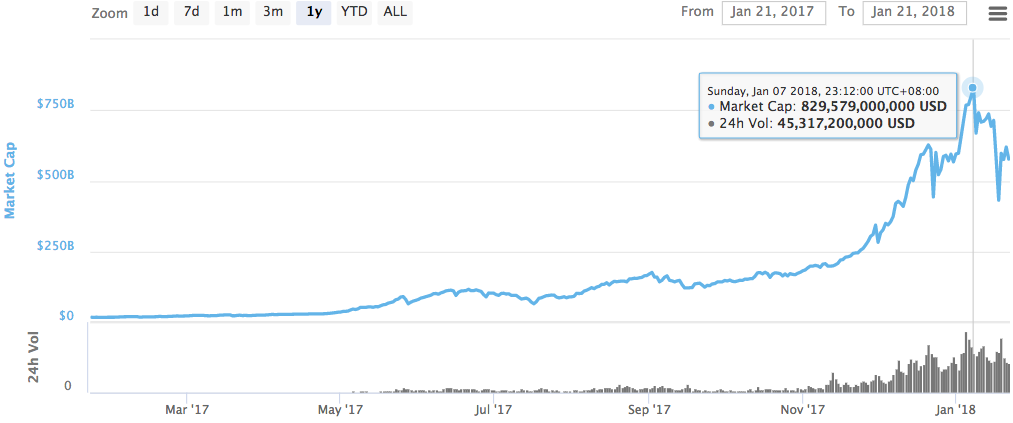
\includegraphics[width = 1\textwidth]{TotalMarketCapitalization.png}
			\caption{2017年1月21日到2018年1月21日期間加密貨幣總市值走勢圖\supercite{CryptocurrencyMarketCapitalizations}}\label{TotalMarketCapitalization}
		\end{figure}

		經由Cryptocurrency Market Capitalizations數據顯示,整體加密貨幣市場自2013年起已經高達150億美金,2014年與2015年間總市值減少到近乎2013年的一半。針對比特幣的價格波動,論文"Have the security flaws surrounding Bitcoin effected the currency's value?."
		\supercite{HavethesecurityflawssurroundingBITCOINeffectedthecurrencysvalue?}
		作出詳盡的市場調研,致力於探討在各個比特幣市場大事件中對比特幣價格的波動影響,針對影響的程度該論文給出影響指數,當中影響最為嚴重的是於2014年2月發生的日本交易所Mt.Gox倒閉事件,因為早期的加密貨幣市場中無完善的法律規範,各國對加密貨幣的接受度有所不同,日本對金融科技的接受度相較於較為開放的情況下成立了全世界第一家比特幣交易所Mt.Gox,也因為交易所不夠普及,使得大部分的加密貨幣交易都集中在Mt.Gox交易所中,使Mt.Gox 倒閉事件成為震盪市場價格重⼤因⼦之⼀,也造成2014與2015年的加密貨幣市場低迷。而在2017年,比特幣又以2016年總市值之35倍的姿態攀上新高點,主要是因為美國最大的期權交易中心芝加哥期權交易所(Chicago Board Options Exchange, CBOE)於2017年12月10日宣布支持比特幣期貨交易,此舉將比特幣價格推升到20,000美金的歷史新高,圖\ref{Thetotalmarketcapitalization}為2013年至2018年歷年的加密貨幣總市值的統計圖表。

			\begin{figure}[!htbp]
				\centering
				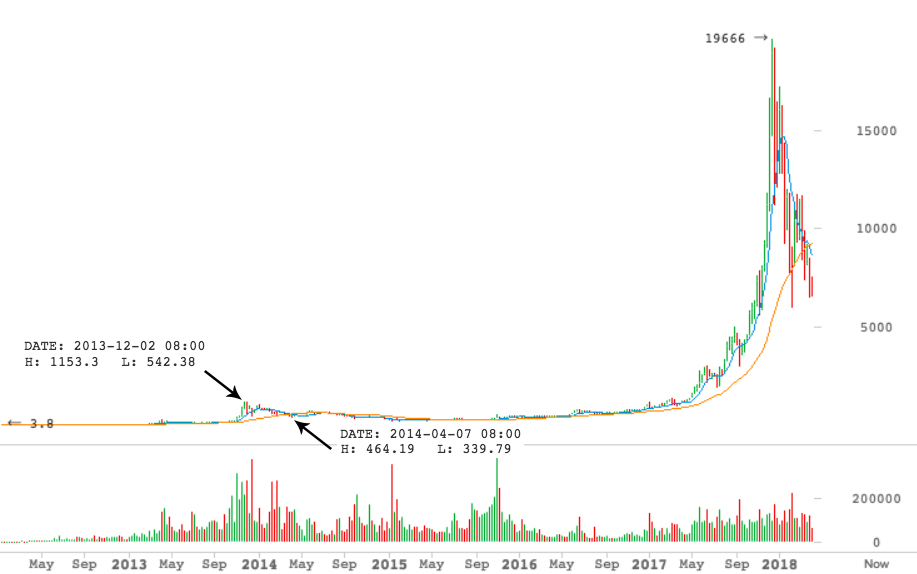
\includegraphics[width = 1\textwidth]{Thetotalmarketcapitalization.jpg}
				\caption{2013年~2018年間比特幣總市值K線圖\supercite{CryptocurrencyMarketCapitalizations}}\label{Thetotalmarketcapitalization}
			\end{figure}
		

			\subsection{加密貨幣的優勢}
			於2009年Satoshi Nakamoto發布了比特幣系統,成為全世界第一個加密貨幣的雛形。其透明的交易信息、區塊鏈交易數據無法修改和刪除、匿名與⾃治系統等特性,促使區塊鏈技術衝破現存傳統中⼼化之⾦融機構技術上的籓籬。以下將逐一說明加密貨幣的七項優點,分別為區塊鏈結算系統不間斷的運行、遠距離支付、貨幣為用戶持有、開放和透明的交易信息、區塊鏈交易數據無法修改和刪除、交易匿名性以及自治性系統。

				第一,區塊鏈結算系統不間斷的運行。基於區塊鏈技術與點對點網絡的架構,以比特幣為例,自2009年至今,所有的比特幣交易事件皆會存儲在比特幣區塊鏈當中,區塊鏈既無法刪除也無法修改,比特幣區塊鏈會以點對點網絡的方式存儲在比特幣網絡中的全節點\supercite{YouReallyShouldRunaBitcoinFullNode:HeresWhy},目前比特幣網絡中的全節點高達10552個。與傳統中心化的銀行數據庫相比,可能會因為銀行的服務器維護,導致交易無法順利進行,甚至可能有黑客的入侵導致銀行或是個人資產有重大的損失。點對點網絡提供穩定的數據庫元數據,不會因為數據庫的停機而無法繼續使用,實現其24小時不間斷之運作。
				
				第二,基於點對點網路架構完成遠距離支付。於跨國匯款從美國轉帳至中國一百萬美金的場景中,需要經過的手續較為繁瑣,資金有可能需要經過多個國家才可以抵達目的地,在經過各個國家的過程中,需要支付各國的手續費,也需要等待各個國家辦理該業務的時間,即使當資金順利抵達了目的地銀行,目的地銀行也需要花將近三至五日的工作日確認該筆金額的來源。屆時領款人亦需要前往銀行核實完整的身份驗證、解釋資金用途,才得以領取這筆跨國資金。比特幣系統當中,有著24小時不間斷運作的優點,也因為點對點網絡架構,使得比特幣無需經由傳統金融機構繁瑣的步驟完成國際匯款,於比特幣系統中無系統壅塞的情況下,平均10分鐘即可入帳,實現其短時間內即可完成遠距離支付之運作。

				第三,加密貨幣為用戶持有。傳統的金融體系中,資金的存儲、流動往往需要經過銀行,用戶將所有的資產存入銀行,拿到的是一串數字的銀行餘額,銀行是一個中心化的機構,有著最高的權利。中央社的新聞\supercite{Bankguardsstolen}指出,臺灣各地於2017年接連於土地銀行、日盛銀行、彰化銀行、京城銀行、兆豐銀行皆傳出銀行行員監守自盜的行為,總金額高達一億三千萬新臺幣。在比特幣系統中,比特幣有如金幣般存放在個人的比特幣地址當中,用戶為真實持有著貨幣,即使是比特幣系統亦無權利動用該筆比特幣資產,唯有比特幣地址的私鑰持有者,才可以轉移該筆比特幣地址中的比特幣資產。

				第四,公開的交易信息。基於區塊鏈架構,所有的交易信息皆以公開的方式存儲於區塊鏈中,並且可信任與方便的取得元數據,以下將針對可信任與元數據進行探討。
				\begin{enumerate}
					\item 可信任:在公有鏈的基本架構上,所有的交易記錄都是公開透明的存儲在區塊鏈當中,比特幣網絡的用戶都可以檢視該筆交易,所有人都可以檢查每個交易記錄的正確性,公開的交易信息亦提升交易數據之可信性。
					\item 元數據:除了以區塊鏈技術為基礎建構出可信任的系統之外,開放和透明的特性讓更多的開發商或新公司得以更容易獲得交易的元數據。畢竟,在傳統金融體系中,所有交易記錄均由中央金融機構存儲,從中央金融機構提取原始交易信息並不容易,區塊鏈的開放性和透明性促使金融公司降低了獲取原始數據努力的門檻。公司或學者可以透過元數據制定出可視化的開發計畫,甚至可以運用大量數據來分析前所未達的新價值觀點。
				\end{enumerate}

				第五,區塊鏈交易數據無法修改和刪除。在區塊鏈結構中,通過嚴格驗證的所有信息都記錄在區塊鏈中,且用戶及系統平台都不賦與刪除及修改之權限。根據區塊鏈的特點,舊區塊的哈希值在連接區塊鏈的過程中,舊區塊的哈希值會被存儲在新區塊。只要區塊中的值被修改,即使僅有1 bit的變化,也會產出完全不同的哈希值,這也就是所謂的雪崩效應(Avalanche effect)\supercite{Theuseofbentsequencestoachievehigher-orderstrictavalanchecriterioninS-boxdesign}。由於上述結構特性,區塊鏈中所有的信息都會被系統紀錄且都不會被改變,倘若區塊中記載的比特幣交易在其中一個比特幣全節點驗證的結果被竄改,則該區塊將不被比特幣系統接受。因此,所有已經存儲在區塊鏈中的交易記錄將不能被修改和刪除,進而實現其架構安全之穩固。

				第六,區塊鏈系統中所有的用戶皆為匿名。現今社會中,個人信息保護已成為企業最重要的課題。在區塊鏈系統中創建的所有帳戶都不會與真實世界中的實體建立直接關聯,也因為沒直接關聯所以建立匿名。區塊鏈系統中的所有帳戶都是由匿名個體創建,匿名的設計可以有效保護消費者的隱私。然而,VISA交易與比特幣系統截然不同,在使用VISA支付系統前,用戶必須向VISA公司的主機提交大量個人信息,這可能會產生個人信息洩露的風險。在區塊鏈技術中,其匿名之特性可以有效地避免這個問題。

				第七,自治系統。在區塊鏈系統中,區塊鏈的運作依賴於一些算法,包括共識算法。因此,在這種自治系統中,沒有人(例如節點或礦工)可以直接改變系統運作的規則。如果在比特幣系統中發現需要更正的嚴重錯誤,可以使用比特幣改進提案(Bitcoin Improvement Proposals,BIP)\supercite{BitcoinImprovementProposals}升級比特幣系統。 在實施比特幣改進提案之前,提議的比特幣改進提案需要得到比特幣系統中超過一定數量的礦工算力支持。由於這種以投票機制升級系統的門檻相當高,使得區塊鏈系統通常不會有大的變化,因為變化不⼤也突顯其相對穩定性。

			\subsection{加密貨幣的劣勢}
			在區塊鏈技術中,有著三項瓶頸,分別為每秒處理的交易量(Transactions Per Second,TPS)僅為七筆的限制、洗錢防治困難、低可擴展性,以下將逐一探討。

				第一,每秒處理的交易量上限僅為7筆。圖\ref{TPS}為國際上較為廣泛使用的⽀付系統之每秒⽀持交易量⽐較圖,以VISA為例,其以公司中心化運營的方式可以支持高達每秒2,000筆交易。但是以區塊鏈技術為基礎的比特幣最大能夠接受的每秒處理交易量僅為7筆。一般認為只要提升區塊大小的限制,就可以提升每秒處理的交易量。提升每秒處理交易量的同時將產生下述的兩項問題,分別為區塊鏈成長速度過快造成節點崩潰以及區塊同步延遲造成區塊鏈分岔:

					\begin{figure}[!htbp]
						\centering
						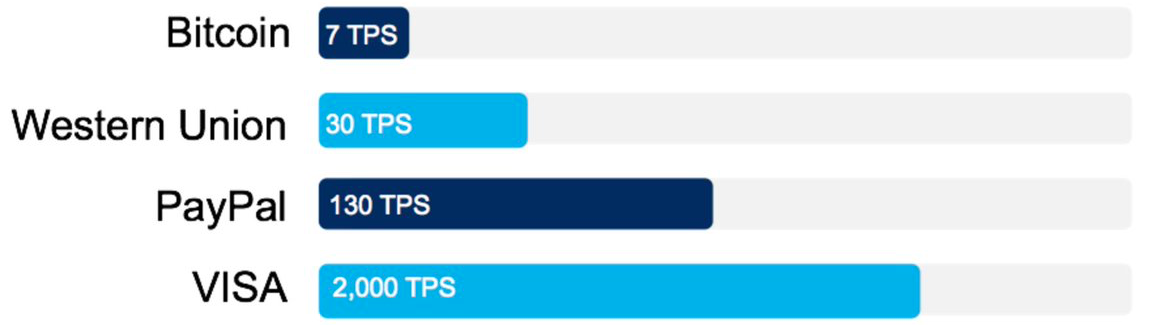
\includegraphics[width = .6\textwidth]{TPS.png}
						\caption{Bitcoin、Western Union\supercite{WesternUnion}、PayPal\supercite{PayPal}以及VISA每秒支持交易量比較圖\supercite{digibyte}}\label{TPS}
					\end{figure}

					\begin{figure}[!htbp]
						\centering
						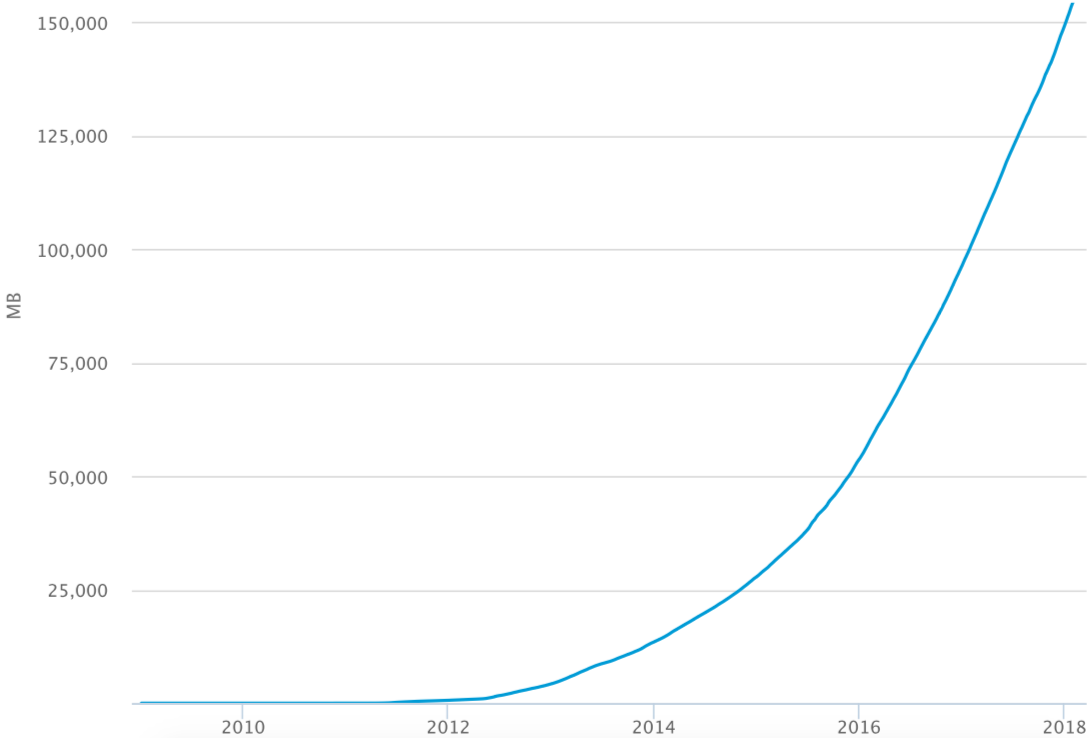
\includegraphics[width = .8\textwidth]{blockchainsize.png}
						\caption{比特幣區塊鏈成長走勢圖\supercite{blockchainsize}}\label{blockchainsize}
					\end{figure}


					\begin{enumerate}
						\item 區塊鏈成⾧速度過快造成節點崩潰。區塊鍊成長速度過快會造成去比特幣全節點不堪負荷:從2009年至今的比特幣區塊鏈大小已達到156GB,這樣的成長速度因為比特幣區塊大小的最大值被設置為1MB。圖\ref{blockchainsize}為過去比特區塊鏈大小,圖中可以發現,於2016年開始,比特幣區塊鏈的成長速度為一直線,這表示著比特幣網絡中持續維持在供不應求的狀況。為解決比特幣每秒⽀持交易量上限的窘迫,現今對⽐特幣的每秒處理交易量有許多優化的⽅案,其中包括解除比特幣區塊大小1MB的限制。在一個區塊上限為1MB的限制下,滿載的比特幣系統中,比特幣區塊鏈平均每十分鐘會增1MB,每小時會增加6MB,每天會增加144MB,每月會增加4.2GB,每年會增加高達50GB,要達到1TB的區塊鏈大小還需要8年,在8年後的未來存儲1TB的數據量應該不會有太大的負擔。倘若解除1MB的區塊限制,在系統的每秒處理交易量看似可以接受更多的交易成倍成長,面臨1TB的比特幣區塊鏈數據會在更短的時間內出現,倘若存儲區塊鏈的成本超過了摩爾定律的成長曲線,會進一步造成用戶自願成為比特幣全節點的意願度降低,使得比特幣網絡的全節點數變少,導致比特幣點對點網絡逐漸轉向中心化網絡發展,失去一開始點對點網絡的意義。

						\item 造成區塊鏈最新區塊同步延遲而使區塊鏈分岔。對於區塊鏈的區塊同步延遲同時也會造成比特幣網絡的影響,J. Göbel於“Increased block size and Bitcoin blockchain dynamics”\supercite{TelecommunicationNetworksandApplicationsConferenceITNAC201727thInternational}有著詳細的研究,在上修區塊大小上限的議題上,用戶因系統占用量提高,⾃願成為⽐特幣全節點意願度下降,此舉可能對⽐特幣點對點網絡建構出的區塊鏈同步上造成延遲,在1055個比特幣全節點當中,平均每十分鐘會有礦工於其中一個全節點生成一個最新的區塊,該最新的區塊會以點對點網絡協議同步到其他1054個節點上。在比特幣系統中,長年來的過程經驗可以發現在礦工生成1MB的區塊後同步到全網節點可以在創造下一個區塊之前完成。倘若將區塊大小修改為2MB或是更大,會使得比特幣全節點的最新區塊同步延遲現象更加明顯,同步延遲會使得區塊鏈分岔,造成1055個比特幣全節點的信息不一致,近一步造成整個比特幣點對點網絡崩潰。
					\end{enumerate}
					

				第二,洗錢防治困難。匿名性為比特幣系統一大特色,比特幣的地址生成的熵是256 bits,亂數是在$2^{256}$的組態空間中隨機選取,這樣的地址與現實生活中的身份並無任何關聯,使得黑市交易、洗錢防治變的困難,甚至有更為前沿的加密貨幣Monero\supercite{noether2014monero}導入了環簽章(Ring Signature)\supercite{Thresholdringsignaturesandapplicationstoad-hocgroups}算法、Zcash\supercite{zhong2002faster}導入零知識證明算法\supercite{Zero-KnowledgeProofsofIdentity},使得原本公開透明的區塊鏈,變得無法檢視,進而造成加密貨幣在洗錢防治上更加的困難。2017年由Thibault de Balthasar and Julio Hernandez-Castro 所提出的論文"An Analysis of Bitcoin Laundry Services."\supercite{AnAnalysisofBitcoinLaundryServices},致⼒探究⽐特幣匿名交易下的資⾦流動模型,試圖以機械學習的方法找出比特幣洗錢模型作為洗錢的工具,圖\ref{Darklaunderworkflow}為該論文針對黑市交易中的洗錢服務運營商Darklaunder進行洗錢機械學習識別有著傑出的成果。

					\begin{figure}[!htbp]
						\centering
						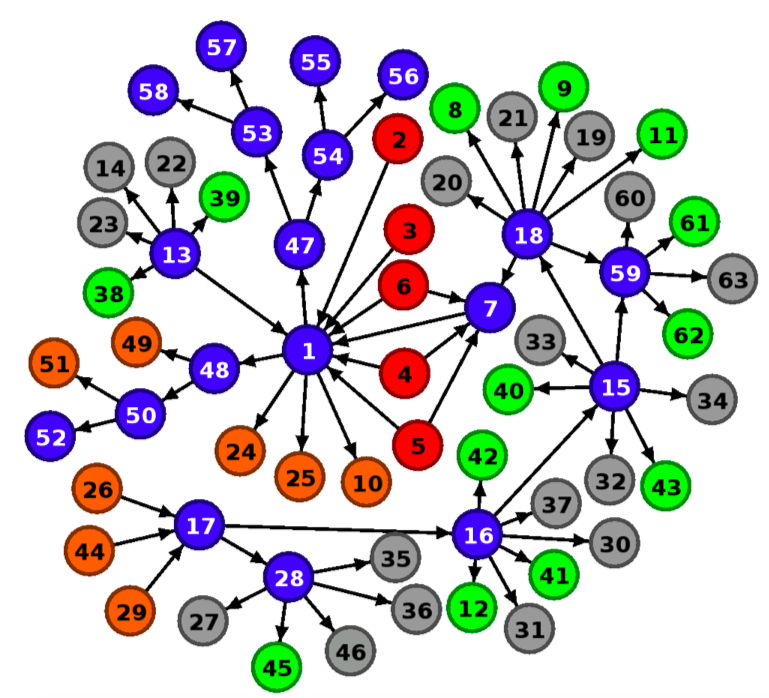
\includegraphics[width = .6\textwidth]{Darklaunderworkflow.png}
						\caption{Darklaunder 洗錢模型\supercite{AnAnalysisofBitcoinLaundryServices}}\label{Darklaunderworkflow}
					\end{figure}

				第三,低可擴展性。區塊鏈架構為了防止各式的攻擊,所以在架構訂定以及接口設計都有著嚴謹的規範。以下將闡述造成比特幣低可擴展性的原因:

					\begin{enumerate}

						\item 修改比特幣協議製作添加外部信息的區塊鏈:比特幣區塊鏈技術是一個嚴謹的架構,倘若要創造可以支持外部信息的結構需要重新創造全新的加密貨幣,大部分的加密貨幣不支持外部輸入,由於外部的信息輸⼊無法保證其信息的正確性,近一步造成垃圾進垃圾出(Garbage In, Garbage Out,GIGO)的問題,倘若錯誤的信息存儲在無法刪除、修改的區塊鏈下,只是強化該筆錯誤信息的錯誤。如食品履歷區塊鏈,致力於將食品生產到超市的過程逐一記錄在區塊鏈上,但如果一開始在輸入信息時,無法保證其信息之正確性,則該食品履歷區塊鏈則毫無意義,錯誤的信息內容甚至可能使該錯誤被強化。

						\item 於區塊頭或交易信息添加外部信息:比特幣區塊鏈上,可以添加一些信息於區塊上,該信息會永久保存於區塊鏈上,除了在區塊上新增信息,在比特幣單筆交易信息上,亦可填寫一些私人信息,但這樣的空間大小有限,且現今的比特幣價格日趨上漲,比特幣交易手續費是以單筆交易大小計算,這將使得在交易中添加些個人信息變得更加昂貴。

					\end{enumerate}

				在比特幣系統中,其區塊鏈僅用於記錄交易記錄,不能擴展更多功能和應用程序。有很多開發者希望將比特幣系統擴展到智能合約等其他應用程序。但是,後來發現改變原始比特幣系統框架是具有挑戰性的工作。因此,全球第二大加密貨幣以太坊(Ethereum,ETH)的作者Vitalik選擇了創建了以太坊虛擬機(Ethereum Virtual Machine,EVM),而非改變原始的比特幣系統框架。以太坊虛擬機所創建的智能合約可以在統一的以太坊平臺上運行,而以太坊也藉此突破了比特幣之技術瓶頸。
	
	\subsection{國際情勢分析}
	\begin{table}[!htbp]
		\centering
		\caption{各國政府對比特幣態度統整表}
		\label{world}
		\begin{tabular}{@{}|l|l|c|c|l|@{}}
		\toprule
		\multicolumn{1}{|c|}{\multirow{2}{*}{序號}} & \multicolumn{1}{c|}{\multirow{2}{*}{國家}} & \multicolumn{2}{c|}{接納} & \multicolumn{1}{c|}{\multirow{2}{*}{禁止}} \\ \cmidrule(lr){3-4}
		\multicolumn{1}{|c|}{} & \multicolumn{1}{c|}{} & 歡迎/放任 & 監管 & \multicolumn{1}{c|}{} \\ \midrule
		1 & 伊朗 & \begin{tabular}[c]{@{}c@{}}監管得當歡迎\\ 比特幣發展\end{tabular} &  &  \\ \midrule
		2 & 以色列 & \begin{tabular}[c]{@{}c@{}}歡迎:欲發展\\ 國際ICO中心\end{tabular} &  &  \\ \midrule
		3 & 法國 & \begin{tabular}[c]{@{}c@{}}放任:與實體\\ 經濟無關\end{tabular} &  &  \\ \midrule
		4 & 美國 & 暫不構成威脅 &  &  \\ \midrule
		5 & 新加坡 & \begin{tabular}[c]{@{}c@{}}不監管但注意\\ 周邊活動\end{tabular} &  &  \\ \midrule
		6 & \begin{tabular}[c]{@{}l@{}}沙特阿拉\\ 伯王国\end{tabular} & \begin{tabular}[c]{@{}c@{}}加密貨幣尚未\\ 成熟,不監管\end{tabular} &  &  \\ \midrule
		7 & 烏克蘭 & 不屬於貨幣 &  &  \\ \midrule
		8 & 韓國 &  & \begin{tabular}[c]{@{}c@{}}很快將監管\\ 交易所\end{tabular} &  \\ \midrule
		9 & 菲律賓 &  & 計劃監管ICO &  \\ \midrule
		10 & 英國 &  & 考慮監管 &  \\ \midrule
		11 & 馬來西亞 & \multicolumn{1}{l|}{} & 正規化監管框架 & \multicolumn{1}{c|}{} \\ \midrule
		12 & 俄羅斯 & \multicolumn{1}{l|}{} & \begin{tabular}[c]{@{}c@{}}2018年7月前\\ 完成立法\end{tabular} & \multicolumn{1}{c|}{} \\ \midrule
		13 & 日本 & \multicolumn{1}{l|}{} & \begin{tabular}[c]{@{}c@{}}任命加密貨幣\\ 監察長\end{tabular} & \multicolumn{1}{c|}{} \\ \midrule
		14 & 香港 & \multicolumn{1}{l|}{} & ICO須受法規監管 & \multicolumn{1}{c|}{} \\ \midrule
		15 & 辛巴威 & \multicolumn{1}{l|}{} &  & \multicolumn{1}{c|}{定法前,屬非法} \\ \midrule
		16 & 摩洛哥 & \multicolumn{1}{l|}{} &  & \multicolumn{1}{c|}{禁止加密貨幣交易} \\ \midrule
		17 & 印尼 & \multicolumn{1}{l|}{} &  & \multicolumn{1}{c|}{\begin{tabular}[c]{@{}c@{}}2018年前\\ 全面禁止\end{tabular}} \\ \midrule
		18 & 中國 & \multicolumn{1}{l|}{} &  & \multicolumn{1}{c|}{禁止加密貨幣} \\ \bottomrule
		\end{tabular}
		\end{table}
	
	比特幣是一種全新的價值交換的媒介,因為區塊鏈技術相當新穎,在各個國家所秉持的態度皆有所不同,大致可將個國家對比特幣的政策分為兩大類,分別為接納與禁止;在接納加密貨幣的分類當中又分為歡迎、放任以及監管。

	在歡迎、放任的政策下的國家包括伊朗、以色列、法國、美國、沙特阿拉伯王國、烏克蘭以及新加坡,上述國家政策上皆已抱持著開放且不監管的方式接納加密貨幣,這些國家認為加密貨幣對於國家金融科技的發展具有前景;在分類於接納但是實施監管的國家中,包括韓國、菲律賓、英國、馬來西亞、俄羅斯、日本以及香港地區皆認為加密貨幣技術可能存在的高風險,且針對加密貨幣的洗錢防制以及非法集資進行嚴格管理,也進一步制定相關的法律,使得國家可以應對新型加密貨幣的糾紛;在禁止加密貨幣的分類中包括辛巴威、摩洛哥、印尼以及中國,這些國家認為比特幣是一個非法的貨幣,因為涉及到洗錢問題、難以實施外匯管制。但是對於區塊鏈技術層面上之探討,在所有國家中都是以蓬勃發展的正面態度看待。上述各國政府對⽐特幣態度如表\ref{world}:

		

	\section{研究目標與內容}
	比特幣在各個國家的蓬勃發展且應用在相當多的領域,應用的領域包括交易所、去中心化交易所、兌幣所、遊戲點數、網路購物、資產的保存、募資以及遠距離支付,甚至是各國的銀行和金融機構都逐步投入人力及資金研究區塊鏈相關技術,甚至是訂定各國相關的法律。在比特幣資產的流動上存在著許多的問題,第一,比特幣的帳戶是由亂數產生器生成,該比特幣帳戶與在現實生活中的用戶並無直接關聯,使得比特幣洗錢變更加盛行。第二,現今的比特幣交易皆為匿名對匿名支付,並無正式的交易憑據開立,使得消費者在購物後,倘若商品存在問題,無法得到法律上的保障。第三,因為比特幣是匿名支付給匿名的交易,使得政府無法從交易行為中進一步課徵稅收,滯礙國家經濟發展。

	本文將解決上述三項問題,設計與實現一個比特幣的實時交易實時监督系统達到下列幾點目標:

		\begin{enumerate}
			\item 導入匿名顧客支付給實名商家的交易模型到加密貨幣交易系統。
			\item 設計與實現在加密貨幣交易中匿名顧客支付給實名商家的交易監督系統;
			\item 於政府端導入多重簽章算法,使比特幣的实时交易监督系统比透過 Green Address 機構驗證更加快速。
			\item 利用多重簽章算法的機制可以讓商家預防比特幣雙重支付的攻擊。
			\item 商家和商品信息管理⼦系統讓商家可進行庫存管理及商家商品管理。
			\item 實現於加密貨幣交易中,消費者匿保持匿名同時也保障消費者權益。
			\item 透過對商家進行實名制,比特幣的交易監督系統讓政府主管機關可以有效獲得稅收。
		\end{enumerate}

	為實現上述目標,本文首先將詳細探討區塊鏈技術的優勢,藉由深度了解區塊鏈技術的優勢可以取之優點,如區塊鏈是一個不間斷、不可竄改、去中心化、公開數據庫、穩定的系統。第二,探討區塊鏈技術的劣勢,區塊鏈技術並非完美,存在著洗錢、逃漏稅、無法保障消費者權益以及交易速度慢的問題,藉由瞭解問題,並設計系統解決。第三,交易模型分析,透過交易模型分析探討在現金、電子貨幣以及加密貨幣存在的交易模型,並在諸多交易模型中發現,匿名支付給實名的交易行為,可以保障消費者隱私,同時保障消費者權益,更使得政府可以對商家的營收進行檢視。第四,系統設計,完成交易分析,並著⼿設計數據庫模型。第五,系統詳細設計與實現,利⽤Java 編程語⾔實現主系統以及三個⼦系統。第六,系統優化,引入比特幣的多重簽章算法,實現比特幣的實時交易監督系統。第七,功能測試,測試以Java編寫程序所有的功能是否能夠完整運作。第八,性能測試,測試在未進行優化的系統與已經優化的系統兩者之間效能的差異。


	\section{論文組織結構}
	在本節中將逐一說明本論文的組織結構共分為七章,分別為緒論、相關理論與技術、系統需求分析、系統概要設計、系統實現、系統測試以及总结与展望:

	第一章:簡述區塊鏈技術解決現有數據庫存在的信息不一致、信息安全問題以及數據庫損毀問題
	。說明在加密貨幣市場中不僅只是比特幣,亦有許多新穎技術為特色的貨幣競爭。簡要探討區塊鏈技術的優點,逐一探討比特幣的缺點及區塊鏈技術瓶頸。最後於研究目標與內容當中,闡述本文的待解決問題以及解決方法。

	第二章:介紹比特幣的發展,闡述比特幣地址生成運用到的算法、生成過程以及多重簽章算法。並詳細說明區塊鏈結構及所有欄位變數與區塊鏈相關的意義。

	第三章:首先對五種交易模型進行分析,進而得知匿名對實名的交易,既可以保障消費隱私且兼具保有消費者權益,並透過需求分析探討本系統需構建的功能模塊。

	第四章:概要設計比特幣交易监督系统的架構,以及說明三個子系統的模塊功能。設計本系統的數據庫結構,設計ER實體聯繫模型 (Entity-relationship model),並闡述本系統的運作流程。最後則將多重簽章算法引入本系統,使得本系統成為比特幣的實時交易监督系统。

	第五章:詳細設計商家和商品信息管理子系統、商家移動裝置收款及交易子系統以及客戶端移動支付和交易子系統的介面。

	第六章:透過功能測試逐一檢視所有功能是否能夠正常運行,經由性能測試分析原始系統與優化後的系統效能之間的差異。

	第七章:說明比特幣區塊鏈系統透過本文所提出之系統,可以達到保障消費者權益同時也兼顧保有顧客隱私,也使得政府可以透過該系統檢視交易明細課徵稅收,而商家亦可對庫存及產品進行管理,達到三贏的局面。
